%Copyright 2014 Jean-Philippe Eisenbarth
%This program is free software: you can
%redistribute it and/or modify it under the terms of the GNU General Public
%License as published by the Free Software Foundation, either version 3 of the
%License, or (at your option) any later version.
%This program is distributed in the hope that it will be useful,but WITHOUT ANY
%WARRANTY; without even the implied warranty of MERCHANTABILITY or FITNESS FOR A
%PARTICULAR PURPOSE. See the GNU General Public License for more details.
%You should have received a copy of the GNU General Public License along with
%this program.  If not, see <http://www.gnu.org/licenses/>.

%Based on the code of Yiannis Lazarides
%http://tex.stackexchange.com/questions/42602/software-requirements-specification-with-latex
%http://tex.stackexchange.com/users/963/yiannis-lazarides
%Also based on the template of Karl E. Wiegers
%http://www.se.rit.edu/~emad/teaching/slides/srs_template_sep14.pdf
%http://karlwiegers.com
\documentclass{scrreprt}
\usepackage{listings}
\usepackage{underscore}
\usepackage[bookmarks=true]{hyperref}
\usepackage[utf8]{inputenc}
\usepackage[english]{babel}
\usepackage{graphicx}
\hypersetup{
    bookmarks=false,    % show bookmarks bar?
    pdftitle={Software Requirement Specification},    % title
    pdfauthor={Emily Longman, Zach Rogers, and Dominic Giacoppe},                     % author
    pdfsubject={Security for Robotics},                        % subject of the document
    pdfkeywords={ROS, Robotics, Security, Capstone}, % list of keywords
    colorlinks=true,       % false: boxed links; true: colored links
    linkcolor=blue,       % color of internal links
    citecolor=black,       % color of links to bibliography
    filecolor=black,        % color of file links
    urlcolor=purple,        % color of external links
    linktoc=page            % only page is linked
}%
\def\myversion{1.0 Final }
\date{}
%\title
\usepackage{hyperref}
\begin{document}

\begin{flushright}
    \rule{16cm}{5pt}\vskip1cm
    \begin{bfseries}
        \Huge{SOFTWARE REQUIREMENTS\\ SPECIFICATION}\\
        \vspace{1.9cm}
        for\\
        \vspace{1.9cm}
        $Security for Robotics$\\
        \vspace{1.9cm}
        \LARGE{Version \myversion approved}\\
        \vspace{1.9cm}
        Prepared by $Emily Longman, Zach Rogers, Dominic Giacoppe$\\
        \vspace{1.9cm}
        \today\\
    \end{bfseries}
\end{flushright}

\tableofcontents

\chapter{Signatures}
\vspace{2in}
\makebox[2.5in]{\hrulefill} \hspace {1.0in}\makebox[2.5in]{\hrulefill} \\
Sponsor \makebox[2.5in][r]{Date} \\

\vspace{.2in}
\makebox[2.5in]{\hrulefill} \hspace {1.0in}\makebox[2.5in]{\hrulefill} \\
Group Member \makebox[2.5in][r]{Date} \\

\vspace{.2in}
\makebox[2.5in]{\hrulefill} \hspace {1.0in}\makebox[2.5in]{\hrulefill} \\
Group Member \makebox[2.5in][r]{Date} \\

\vspace{.2in}
\makebox[2.5in]{\hrulefill} \hspace {1.0in}\makebox[2.5in]{\hrulefill} \\
Group Member \makebox[2.5in][r]{Date} \\


\chapter{Introduction}

\section{Purpose}
$<$To define the requirements and deliverables for (team name)'s capstone project to our sponsor, Vedanth Narayanan.$>$

\section{Scope}
$<$We are to find security vulnerabilities in ROS/SROS, document these vulnerabilities, and if possible, produce patches for anything we find. Any patches produced will be submitted to the ROS project. Our testing will be focused around ROS/SROS running on a drone, and we will see if we can compromise that drone based on our findings.$>$

\section{Definitions}
\begin{itemize}
  \item Vulnerability: Any exploitable piece of code or system that would allow unauthorized users to interact with/damage/control the system, especially in a malicious manner.
  \item ROS: Robot Operating system, as found at link
  \item SROS: Secure ROS; a project based on ROS with the goal of implementing various security standards.
\end{itemize}

\section{References}
$<$blah blah blah$>$

\section{Overview}
$<$blah blah blah$>$


\chapter{Overall Description}

\section{Product Perspective}
$<$All software developed by (Team name) should have 2 objectives:
1. Fixing a specific, known vulnerability in ROS/SROS
2. Be lightweight enough that the implementation doesn't drastically affect the overall operation of the robot. Ideally, any code produced would be later incorporated into ROS itself, and not an external layer or program.$>$

\section{Product Functions}
$<$blah blah blah$>$

\section{User Characteristics}
$<$blah blah blah$>$

\section{Constraints}
$<$blah blah blah$>$

\section{Assumptions and Dependencies}
$<$blah blah blah$>$

\section{Apportioning of Requirements}
  \begin{center}
    \begin{figure}
      \makebox[\textwidth]{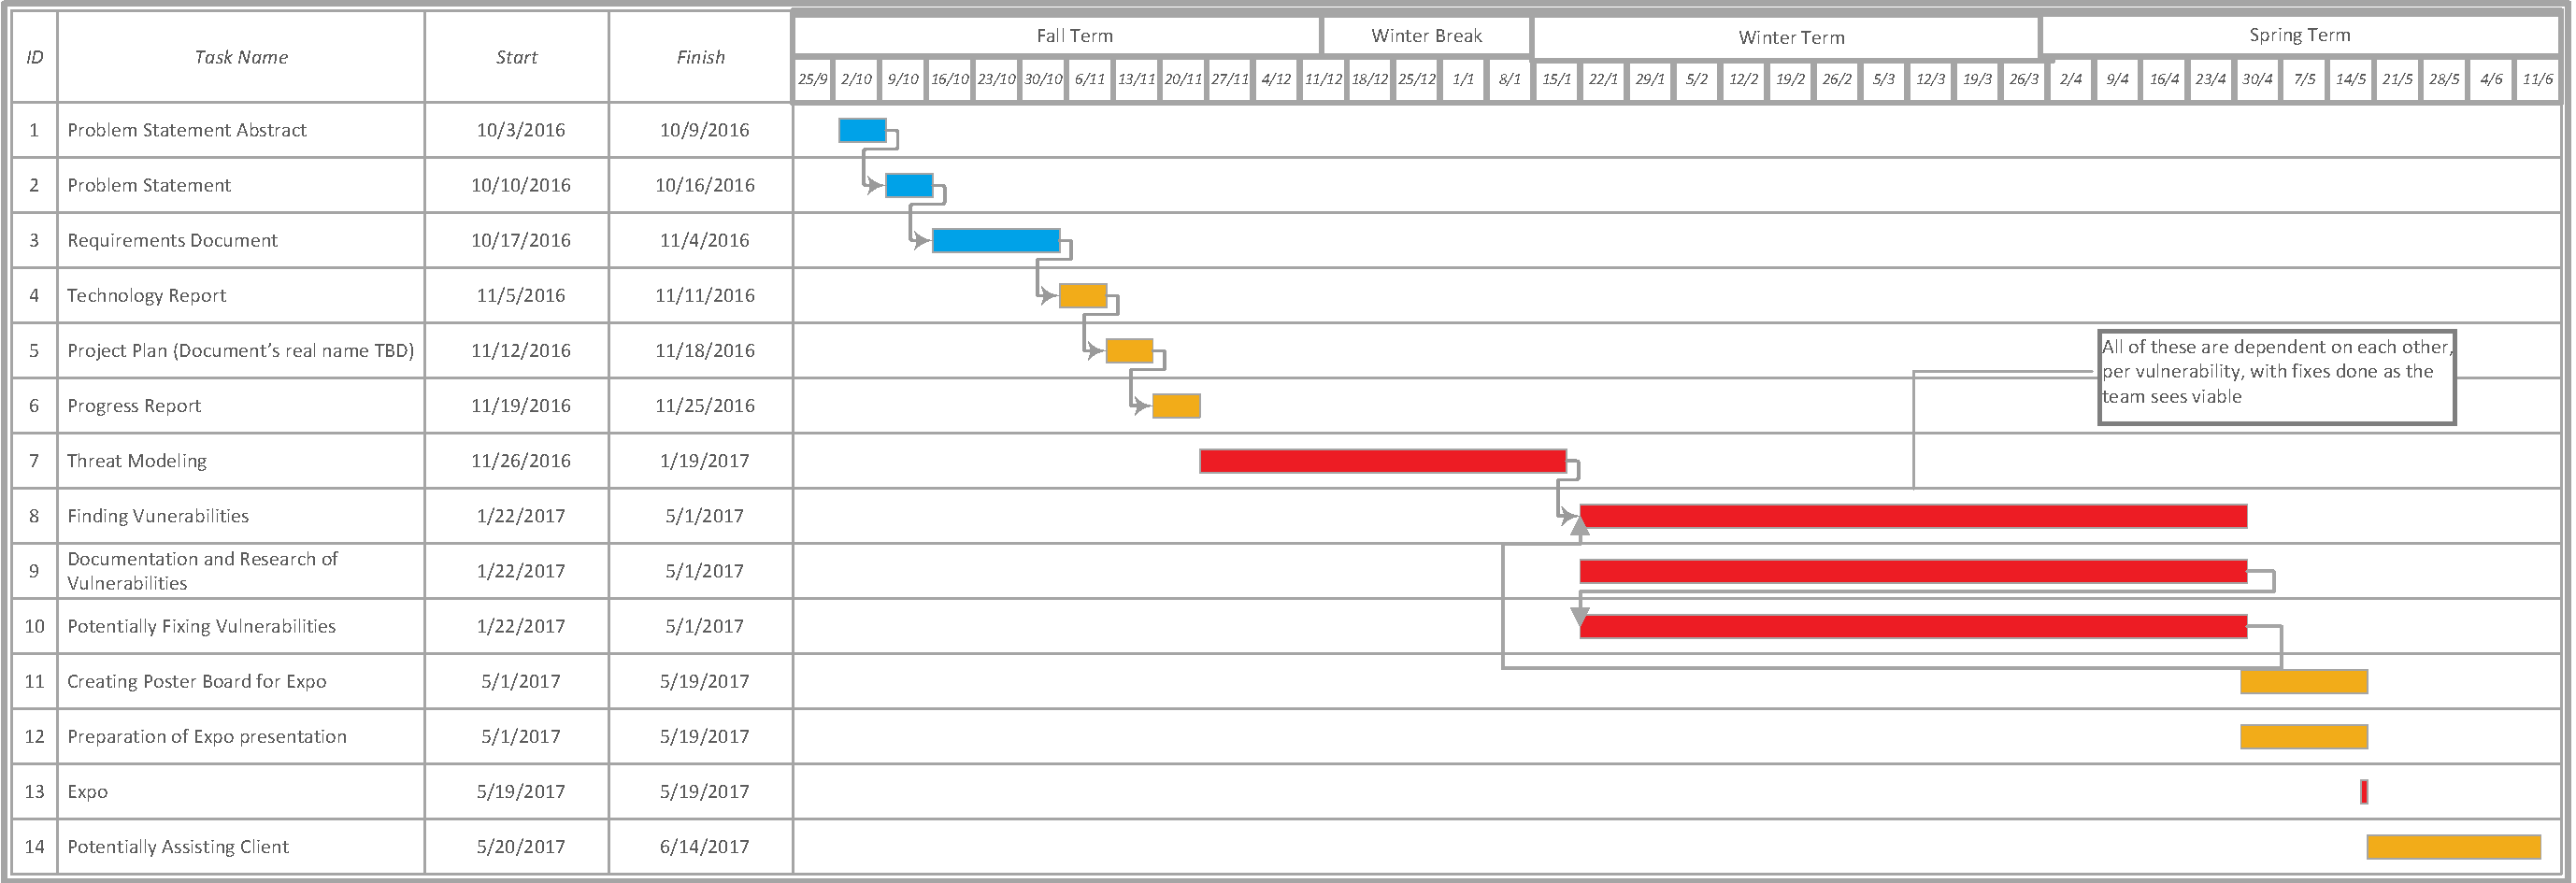
\includegraphics[width=\paperwidth]{ganntSPnotext.png}}
      \caption{Gantt Chart}
      \label{fig:gantt}
    \end{figure}
  \end{center}


\chapter{Specific Requirements}

\section{Software Interfaces}
$<$As we are looking for vulnerabilities in ROS, all code produced must be compatible with it or integrated into it. The version of ROS we will be using is Kinetic Kame, the current long-term support version of ROS.$>$

\subsection{Communications Protocol}
$<$ROS uses 2 major forms of communication. Internally, ROS has the publisher subscriber system, which works basically like a socket system.
Publishers export data, and anyone who subscribes to that publisher receives the data, with no limit to the number of
subscribers or any authentication on who can subscribe. There is also normally some sort of wireless/wired connection to a base
station, which controls the starting and stopping of the robot. These generally take the form of a standard LAN connection,
although with extra effort more complicated setups are possible. (SOURCE)$>$

\section{External Interfaces}
$<$The external interface we will be working with is a DJI FlameWheel 550 hexcopter. 
Included on it is a beaglebone black with a pixhawk firecap mounted on it. 
The sensors it has are the same as that of a regular pixhawk, which includes a gps and 9DOF.$>$

\section{Functions}
$<$Any vulnerabilities found should in some way compromise the functionality or integrity of the robot. In turn, any fixes created for said vulnerabilities should prevent those from being compromised.$>$

\section{Specific Requirements}
$<$As previously stated, at the moment (Team Name) is in the process of finding specific vulnerabilities. When we do find one, we will produce documentation outlining at least but not limited to:
Our operating environment, the type of attack, the particular system/piece of code attacked, the success rate of the attack, the result of the attack, and the potential fix to prevent the attack.$>$

\section{Software Attributes}
  \subsection{Reliability}
  $<$blah blah blah$>$

  \subsection{Availability}
  $<$blah blah blah$>$

  \subsection{Security}
  $<$blah blah blah$>$

  \subsection{Maintainability}
  $<$blah blah blah$>$

  \subsection{Portability}
  $<$blah blah blah$>$


\end{document}
